%!TeX root=../main.tex

\begin{figure}[th!]
\vskip -0.05in % useful knobs to optimize layout
    \centering        
    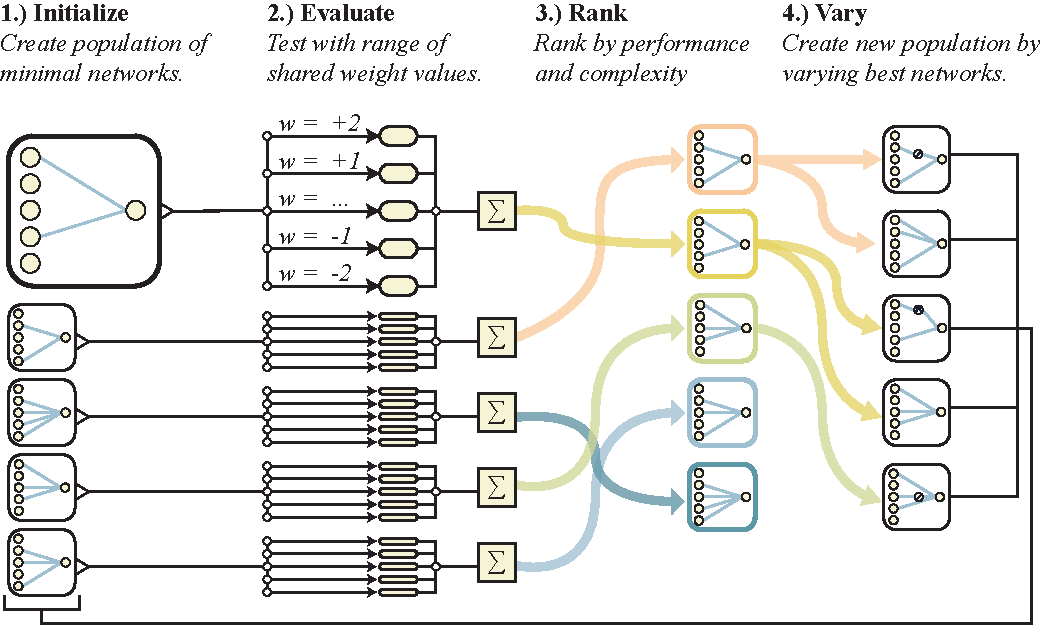
\includegraphics[width=1\textwidth]{img/wann.pdf}   
\vskip -0.05in % useful knobs to optimize layout
    \caption      
    {     
        \textit{Overview of Weight Agnostic Neural Network Search}
        \newline
        Weight Agnostic Neural Network Search avoids weight training while exploring the space of neural network topologies by sampling a single shared weight at each rollout. 
        %
        Networks are evaluated over several rollouts. At each rollout a value for the single shared weight is assigned and the cumulative reward over the trial is recorded. 
        %
        The population of networks is then ranked according to their performance and complexity. 
        %
        The highest ranking networks are then chosen probabilistically and varied randomly to form a new population, and the process repeats.
    }         
    \label{fig:overview}
\vskip -0.15in % useful knobs to optimize layout
\end{figure}

